\documentclass[12pt, letterpaper]{article}
\usepackage[utf8]{inputenc}
\usepackage{indentfirst}
\usepackage{graphicx}
\usepackage{algorithm}
\usepackage{algpseudocode}
\usepackage{float}
\usepackage{blindtext}
\usepackage{hyperref}

\hypersetup{
    colorlinks=true,
    linkcolor=,
    filecolor=magenta,      
    urlcolor=cyan,
    pdftitle={Trabalho 2 - MC920},
    pdfpagemode=FullScreen,
    pdfsubject={Binarização de imagens com diferentes métodos},
    pdfauthor={Rian Radeck Santos Costa},
    pdfkeywords={binarization, image, method}
    }

\graphicspath{ {images/} }

\title{Trabalho 2 - MC920}
\author{Rian Radeck Santos Costa - 187793}
\date{27 de Setembro de 2022}
\renewcommand*\contentsname{Sumário}

\begin{document}

\maketitle
\newpage
\tableofcontents
\newpage

\section{Especificações do programa}
    Todas as imagens na pasta desse trabalho (./binary\_images) foram geradas com vizinhança 5 x 5 e os valores padrões sugeridos, exceto quando existe um arquivo de texto com os valores utilizados.
    
    Notei algumas coisas sobre esse trabalho:
    \begin{itemize}
        \item{Valores altos (entre 15 e 50) para vizinhança geralmente funcionam melhor.}
        \item{Os valores de $k$ são como uma tolerância para bordas e ruídos.}
        \item{O método de Bernsen é o mesmo que o método do contraste com objeto e fundo invertidos.}
        \item{Foi pedido que fossem gerados histogramas para as imagens binárias, porém isso nos daria a mesma informação da porcentagem de preto delas, sendo assim fiz os histogramas das imagens originais, o que nos fornece a informação do contraste das imagens.}
        \item{Os $k$'s não deveriam ser negativos para que o ``objeto'' da imagem (e.g. texto) continue preto?}
    \end{itemize}
    
    Encorajo fortemente também que o código seja executado para uma melhor visualização das imagens e um melhor entendimento sobre os parâmetros dos métodos apresentados, principalmente dos métodos mais complexos e da aproximação contínua dos histogramas.
    Enfim, esclarecidos os passos iniciais vou mostrar as imagens que melhor se encaixaram em cada método e suas porcentagens de preto. 

\section{Algoritmos}
    Todos os métodos foram implementados de maneira similar, mudando somente a maneira que é calculado o limiar para cada pixel.

    A implementação ficou bem simples: para cada pixel era considerada uma vizinhança de $n$ x $n$ centrada nele, feita com slicing em python. Caso o slicing caísse fora dos limites de altura e largura da imagem, seus valores eram ``clipados'' para os limites, ou seja, nem sempre a vizinhança era $n$ x $n$, por exemplo para o pixel $(0, 0)$ o tamanho de sua vizinhança era aproximadamente $\frac{1}{4}$ do tamanho da vizinhança de pixeis mais centralizados. Algo também a ser notado é que quando $n$ é par, ele é arredondado para cima, por exemplo uma vizinhança 2 x 2 é na verdade uma vizinhança 3 x 3.

    Segue um pseudocódigo da implementação desses algoritmos:
    \begin{algorithm}
    \caption{Generic Algorithm $(img, n)$}
    \begin{algorithmic}
        \State {new\_img $\gets img$}
        \For{$i \gets 0 \ldots img$.height$- 1$}
            \For{$j \gets 0 \ldots img$.width$- 1$}
                \State {start\_row $\gets max(0, i - \left\lfloor\frac{n}{2}\right\rfloor)$}
                \State {end\_row $\gets min(img$.height$, i + \left\lfloor\frac{n}{2}\right\rfloor)$}
                \State {{start\_column $\gets max(0, j - \left\lfloor\frac{n}{2}\right\rfloor)$}}
                \State {end\_column $\gets min(img$.width$, j + \left\lfloor\frac{n}{2}\right\rfloor)$}
                \\
                \State {neighbourhood $\gets img$[start\_row$\ldots$end\_row][start\_column$\ldots$end\_column]}
                \State {threshold $\gets$ GivenMethod(neighbourhood)}

                \If{$img[i][j] >$ threshold}
                    \State {new\_img[i][j] $\gets$ Object}
                \Else
                    \State {new\_img[i][j] $\gets$ Background}
                \EndIf
            \EndFor
        \EndFor
        \\
        \Return {new\_img}
    \end{algorithmic}
    \end{algorithm}

    Os cálculos feitos pela função GivenMethod foram os fornecidos no enunciado do trabalho. 

    OBS: Note que no método de Phansalskar, More e Sabale, os valores são divididos por 255 (normalizados) antes que seja feito o cálculo do limiar.

\newpage
\section{Método Global}
    Considerando a simplicidade e velocidade de execução desse método (não considera vizinhança), acho que ele melhor se encaixa mostrando onde se encaixam as sombras de uma imagem. Observe na imagem das pimentas
    \begin{figure}[H]
        \centering
        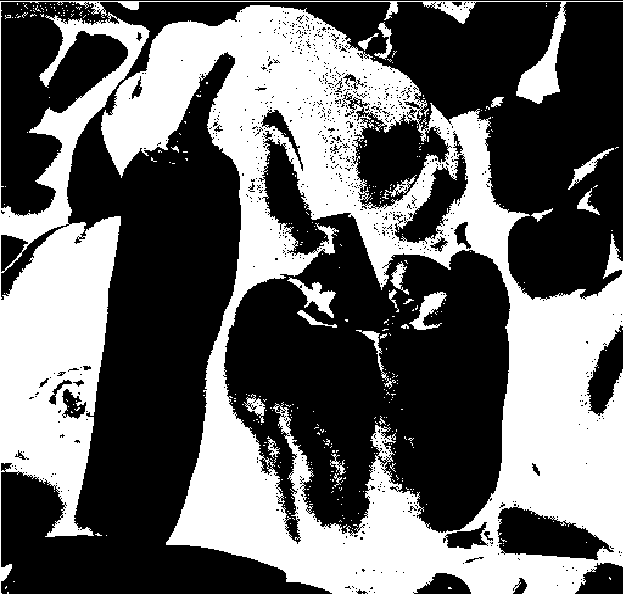
\includegraphics[width=0.6\textwidth]{global_peppers.png}
        \\{Método Global ($T = 100$)}

        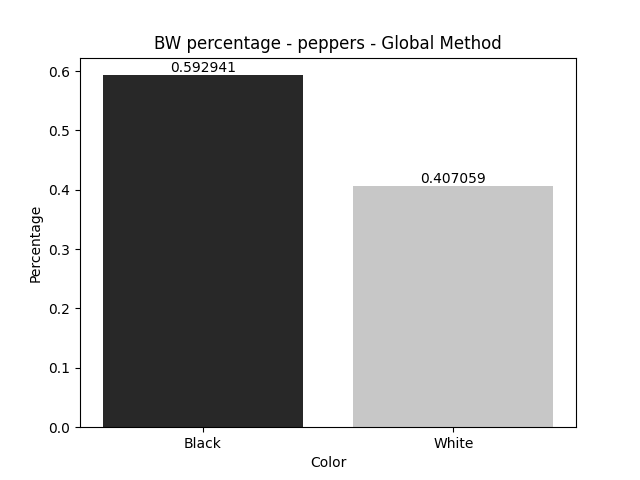
\includegraphics[width=0.69\textwidth]{global_peppers_bw_percentage.png}
        \\{Porcentagem da coloração da imagem binária}
    \end{figure}
    Veja que é bem claro onde estão as sombras da imagem, ainda mais que essa é uma imagem de contraste razoável, como é possível ver em \ref{hist:peppers}.


\section{Método de Bernsen}
    Gostei bastante do resultado obtido no Fiducial com $n = 25$. Os quadrados ficaram bem separados e definidos dada a simplicidade do método, além de que a parte escura da imagem foi bem processada.
    \begin{figure}[H]
        \centering
        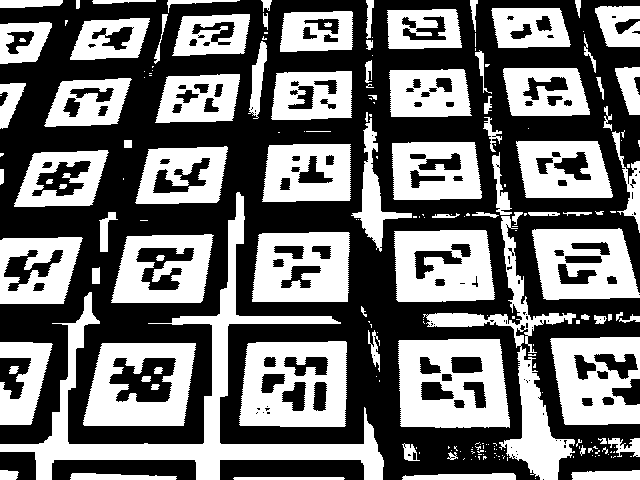
\includegraphics[width=0.6\textwidth]{bernsen_fiducial.png}
        \\{Método de Bernsen ($n = 25$)}

        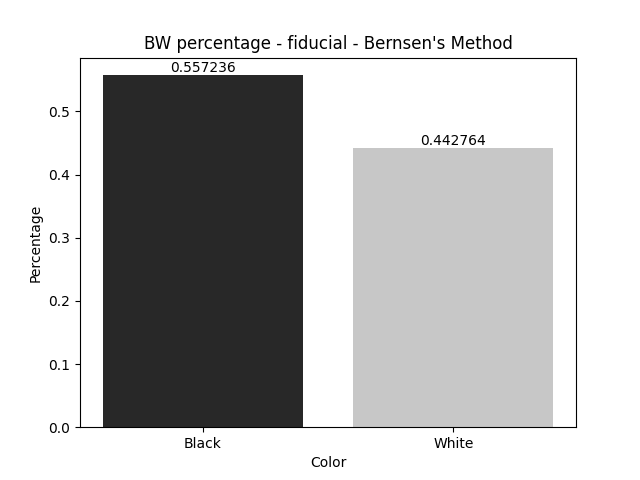
\includegraphics[width=0.69\textwidth]{bernsen_fiducial_bw_percentage.png}
        \\{Porcentagem da coloração da imagem binária}
    \end{figure} 
    Claramente, o método do Contraste fornecerá um resultado similar, o que faz sentido, já que essa imagem tem um baixo-médio nível de contraste, como podemos ver em \ref{hist:fiducial}.

\section{Método de Niblack}
    É um método muito interessante, já um pouco mais complexo. Notei que em áreas de cor uniforme existia bastante ruído, dessa forma fui observando que era uma boa maneira de identificar fontes de luz, o que fica bem evidente no exemplo a seguir
    \begin{figure}[H]
        \centering
        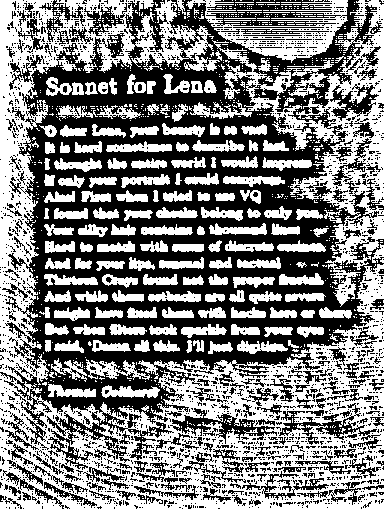
\includegraphics[width=0.7\textwidth]{niblack_sonnet.png}
        \\{Método de Niblack ($n = 25; k = 0,1$)}
    \end{figure}
    \begin{figure}[H]
        \centering
        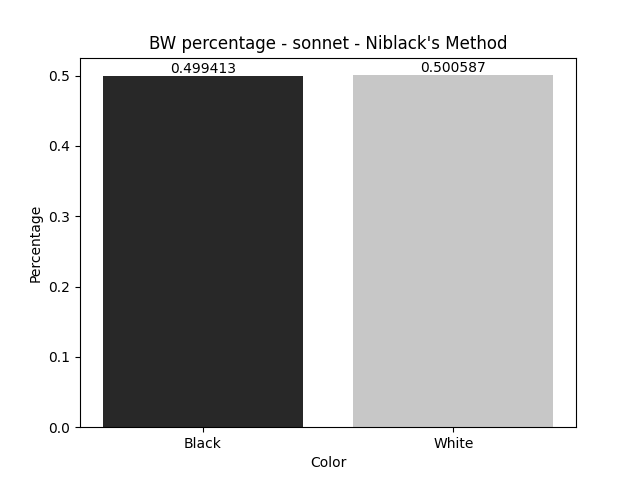
\includegraphics[width=0.8\textwidth]{niblack_sonnet_bw_percentage.png}
        \\{Porcentagem da coloração da imagem binária}
    \end{figure}
    Claro que isso é só uma observação menor no método de Niblack; esse método é na verdade um dos métodos pioneiro na binarização de imagens e funciona muito bem em textos e imagens onde o fundo não é uniforme em geral.

    Esse método também mostra um resultado bem interessante com o wegde, acredito que uma imagem de bom contraste seja fundamental já que uma propagação de luz cria um degradê de contraste, podemos observar o histograma de contraste do sonnet em \ref{hist:sonnet}.

\section{Método de Sauvola e Pietaksinen}
    Realmente um método mais complexo e adaptável para binarização de imagens, aqui é possível obter filtragens bem precisas de diversos fatores da imagem (e.g. bordas), como é possível observar na seguinte imagem
    \begin{figure}[H]
        \centering
        
\includegraphics[width=0.7\textwidth]{sauvola_wedge.png}
        \\{Método de Sauvola e Pietaksinen ($n = 27; k = 0,12; R = 72$)}

        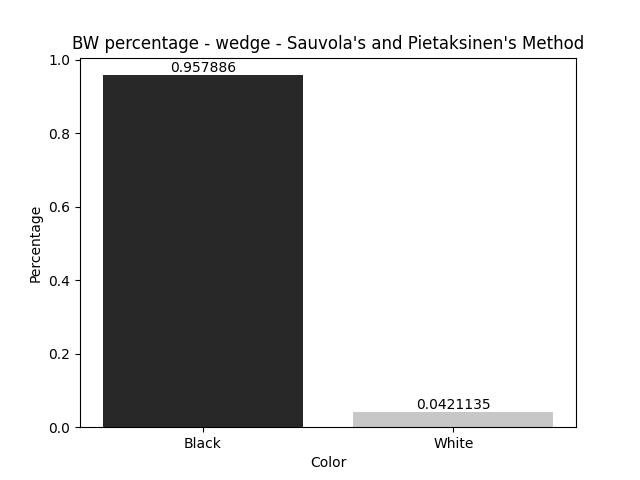
\includegraphics[width=0.69\textwidth]{sauvola_wedge_bw_percentage.png}
        \\{Porcentagem da coloração da imagem binária}
    \end{figure}
    Vemos que é bem fácil distinguir formas na imagem, e claro, vai funcionar muito bem com textos e formas simples como no fiducial e no sonnet, já que objeto e fundo são facilmente definidos por identificações ``mais humanas'' (as formas da imagem).

\section{Método de Phansalskar, More e Sabale}
    Sendo um método refinado do método de Sauvola e Pietaksinen, ele apresentará resultados similares, com mais opções de refinamento permitindo que sejam atingidos resultados espetaculares para a binarização de imagens, com pouquíssima perca de detalhes e grande precisão na identificação de mudança de contextos.
    \begin{figure}[H]
        \centering
        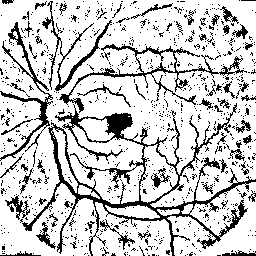
\includegraphics[width=0.6\textwidth]{phansalskar_retina.png}
        \\{Método de Phansalskar, More e Sabale ($n = 25; k = -0,12; R = 0,6; p = 1; q = 100$)}
    \end{figure}
    \begin{figure}[H]
        \centering
        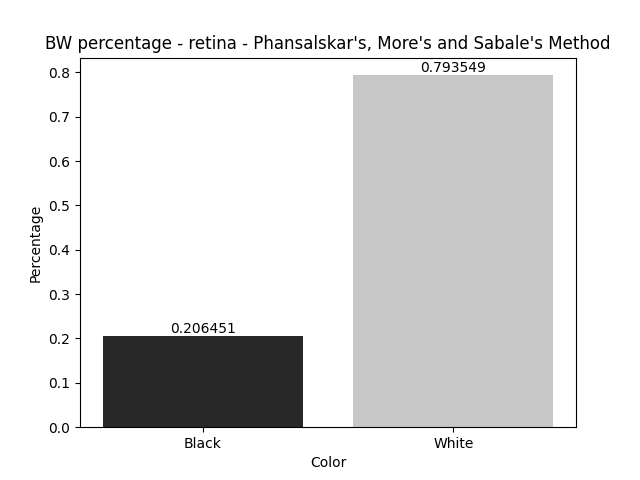
\includegraphics[width=0.8\textwidth]{phansalskar_retina_bw_percentage.png}
        \\{Porcentagem da coloração da imagem binária}
    \end{figure}
    Observe que é muito interessante a maneira que esse método consegue separar os traços da retina de maneira muito boa (claro que meus parâmetros não são os melhores), acredito que com um refinamento melhor seja possível eliminar todo o ruído e manter somente os traços da retina. Inclusive esse método foi criado em um contexto de estudar citologia e lendo o artigo \href{https://www.researchgate.net/publication/224226466_Adaptive_local_thresholding_for_detection_of_nuclei_in_diversity_stained_cytology_images}{Adaptive Local Thresholding for Detection of Nuclei in Diversely Stained Cytology Images - Neerad Phansalkar, Sumit More, Ashish Sabale, Dr. Madhuri Joshi} fiquei realmente surpreso o quão melhor seus resultados foram em relação ao método de Sauvola e Pietaksinen.

\section{Métodos de Contraste, Média e Mediana}
    Como já mencionado, o método de contraste é muito similar ao método de Bernsen e se encaixa em aplicações bem parecidas (e.g. QR codes, imagens OCT). 

    O método da média acaba sendo bem útil uma vez que ele é um método de suavização de imagens, ele funciona reduzindo a quantidade de variação de intensidade entre pixeis próximos e geralmente é utilizado para reduzir ruído de uma imagem.

    O método da mediana é um filtro de ruído, assim como o da média, porém geralmente faz um trabalho mais limpo de desejado no quesito de preservar qualidade e detalhes da imagem.

    Leitura sobre o método de Bernsen / Contraste: \href{https://www.researchgate.net/publication/315751159_Implementation_of_Bernsen's_Locally_Adaptive_Binarization_Method_for_Gray_Scale_Images}{Implementation of Bernsen’s Locally Adaptive Binarization Method for Gray Scale Images - Can Eyupoglu}

    Leitura sobre o método da média: \href{https://homepages.inf.ed.ac.uk/rbf/HIPR2/mean.htm}{HIPR2 - Mean Filter}

    Leitura sobre o método da mediana: \href{https://homepages.inf.ed.ac.uk/rbf/HIPR2/median.htm}{HIPR2 - Median Filter}


\newpage
\section{Histogramas}
    \subsection{Fiducial}
        Aqui temos uma imagem de baixo contraste (maioria dos pixeis menores que 80), apesar de existir uma grande concentração na porção direita do histograma, isso se deve a grande quantidade de detalhes pretos dos códigos na imagem e não a uma boa distribuição de contraste da imagem.
        \begin{figure}[H]
            \label{hist:fiducial}
            \centering
            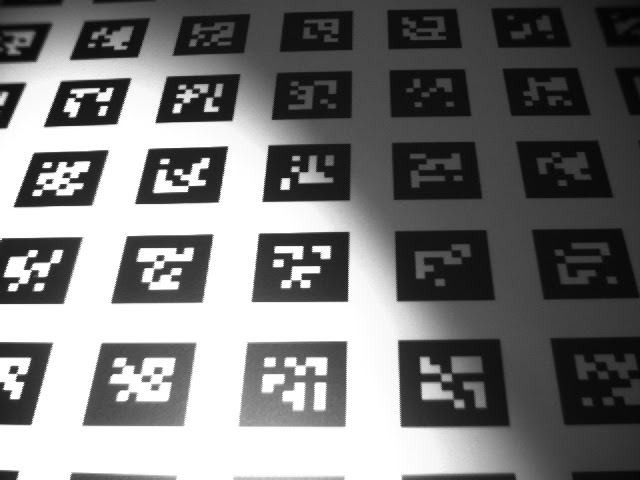
\includegraphics[width=0.6\textwidth]{fiducial.png}
            \\{Imagem original}

            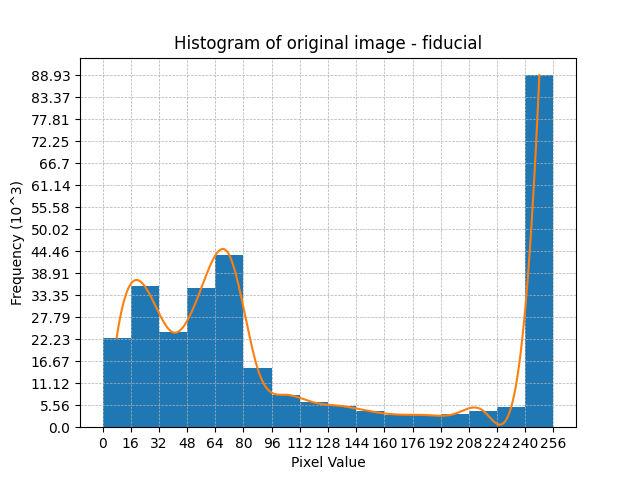
\includegraphics[width=0.74\textwidth]{fiducial_histogram.png}
            \\{Histograma de Contraste}
        \end{figure}
    \subsection{Peppers}
        Aqui temos uma imagem de médio contraste, com uma maior concentração no centro do histograma, tornando uma boa imagem para identificação de sombras e detalhes.
        \begin{figure}[H]
            \label{hist:peppers}
            \centering
            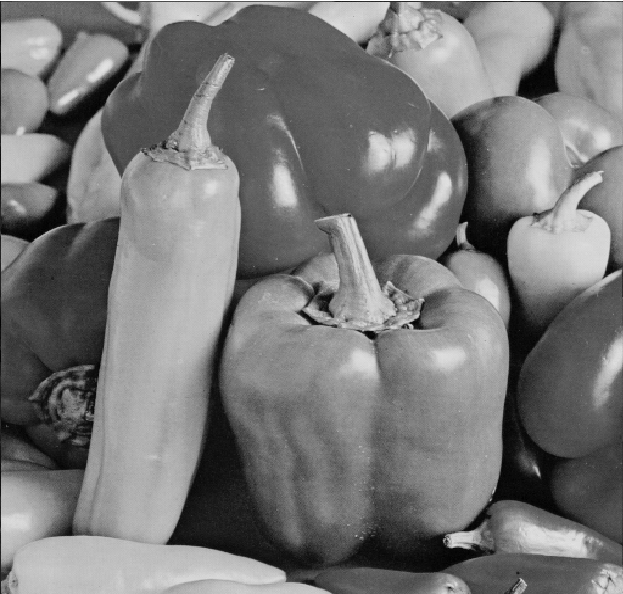
\includegraphics[width=0.6\textwidth]{peppers.png}
            \\{Imagem original}

            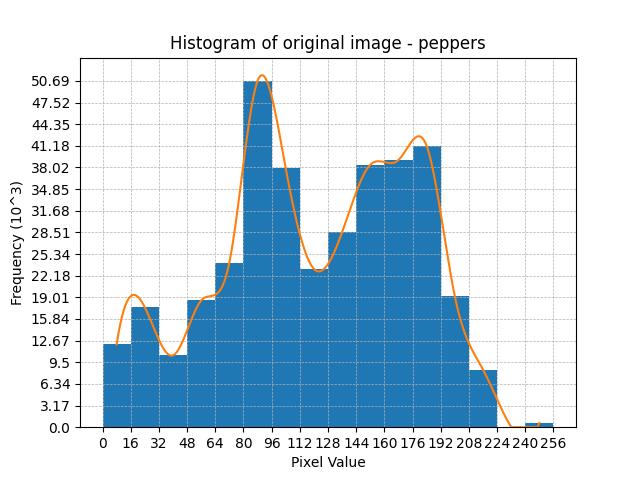
\includegraphics[width=0.74\textwidth]{peppers_histogram.png}
            \\{Histograma de Contraste}
        \end{figure}
    \subsection{Sonnet}
        Vemos um excelente exemplo de alto contraste nessa imagem, apesar da presença de texto os níveis de cinza estão bem distribuídos.
        \begin{figure}[H]
            \label{hist:sonnet}
            \centering
            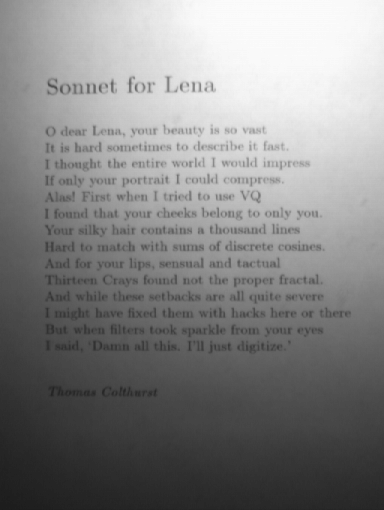
\includegraphics[width=0.5\textwidth]{sonnet.png}
            \\{Imagem original}

            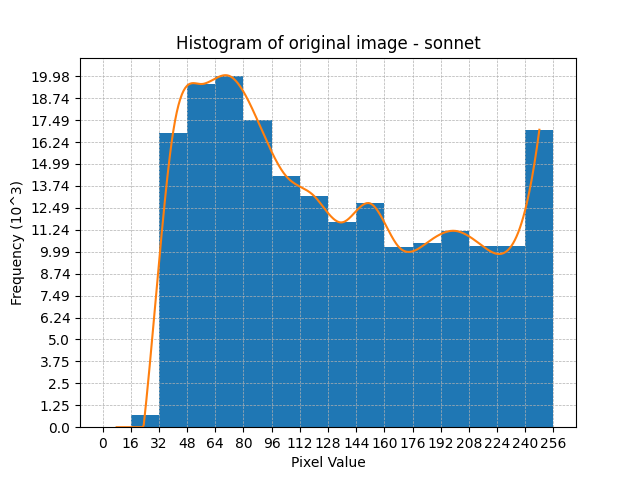
\includegraphics[width=0.65\textwidth]{sonnet_histogram.png}
            \\{Histograma de Contraste}
        \end{figure}
    \subsection{Baboon}
        Outro bom exemplo de alto contraste nessa imagem.
        \begin{figure}[H]
            \label{hist:baboon}
            \centering
            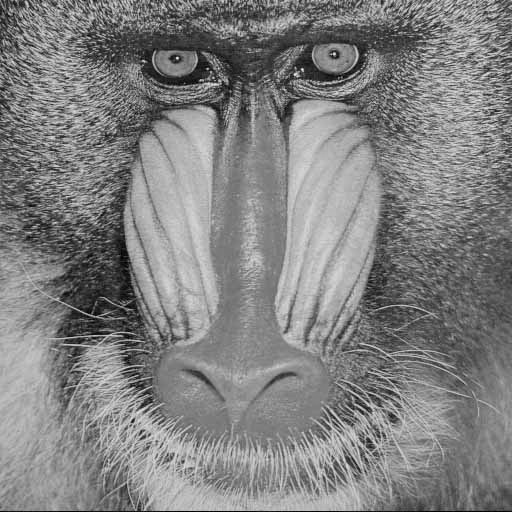
\includegraphics[width=0.6\textwidth]{baboon.png}
            \\{Imagem original}

            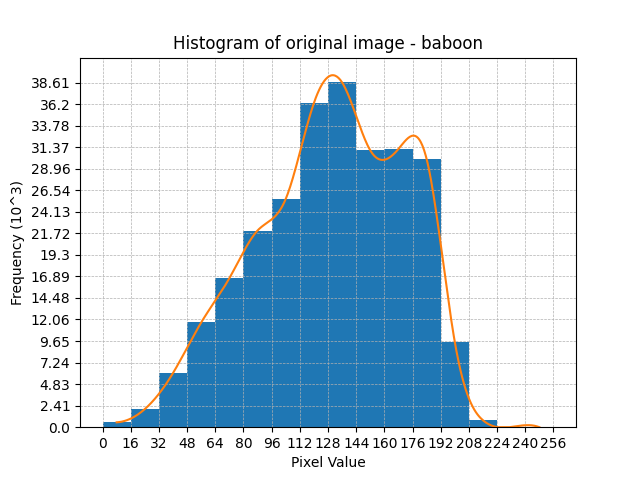
\includegraphics[width=0.74\textwidth]{baboon_histogram.png}
            \\{Histograma de Contraste}
        \end{figure}
    \subsection{Monarch}
        \begin{figure}[H]
            \label{hist:monarch}
            \centering
            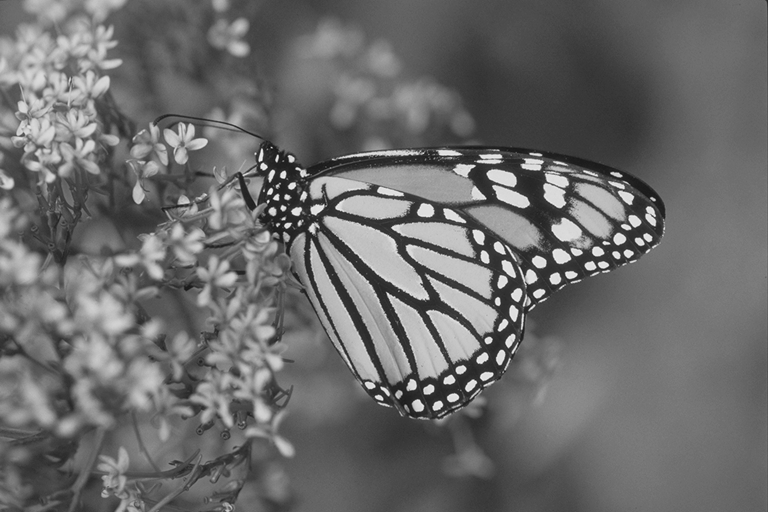
\includegraphics[width=0.7\textwidth]{monarch.png}
            \\{Imagem original}

            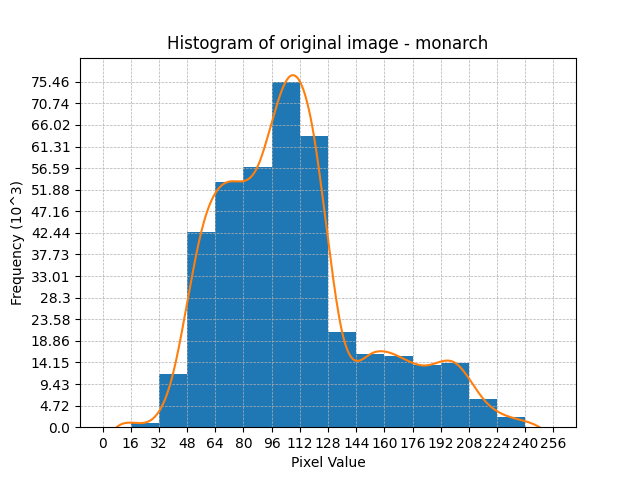
\includegraphics[width=1\textwidth]{monarch_histogram.png}
            \\{Histograma de Contraste}
        \end{figure}
    \subsection{Retina}
        \begin{figure}[H]
            \label{hist:retina}
            \centering
            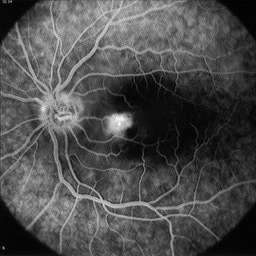
\includegraphics[width=0.5\textwidth]{retina.png}
            \\{Imagem original}

            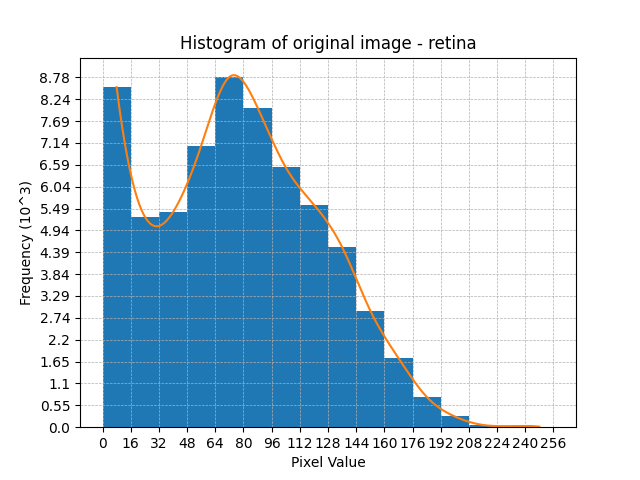
\includegraphics[width=0.9\textwidth]{retina_histogram.png}
            \\{Histograma de Contraste}
        \end{figure}
    \subsection{Wedge}
        \begin{figure}[H]
            \label{hist:wedge}
            \centering
            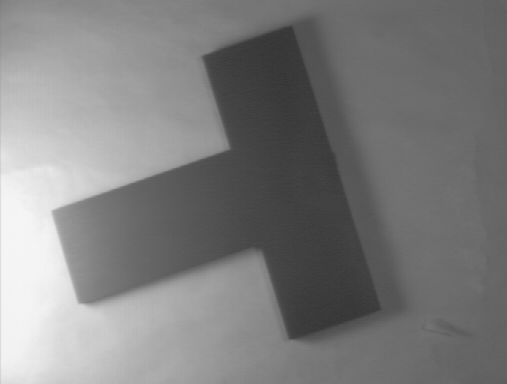
\includegraphics[width=0.6\textwidth]{wedge.png}
            \\{Imagem original}

            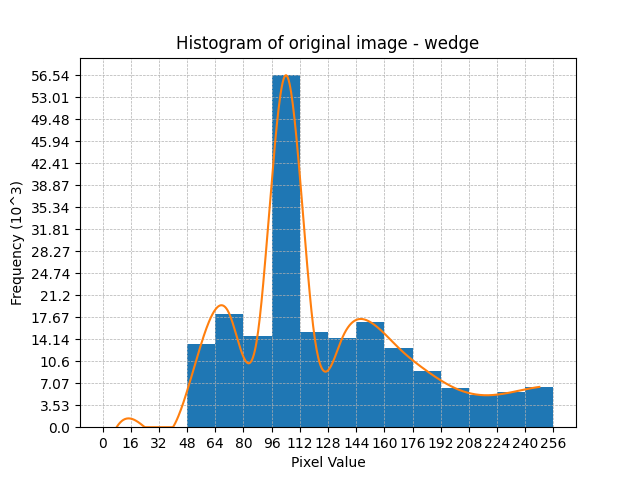
\includegraphics[width=0.9\textwidth]{wedge_histogram.png}
            \\{Histograma de Contraste}
        \end{figure}

\end{document}